% latex template. https://www.overleaf.com/latex/templates/kantonsschule-wattwil-maturaarbeit-template
\RequirePackage[l2tabu, orthodox]{nag}
\documentclass[a4paper,openright]{scrreprt} % evtl twoside
\usepackage[utf8]{inputenc}
\usepackage[ngerman,english]{babel}
\usepackage[autostyle=true,german=quotes]{csquotes}
\usepackage{scrhack}
\usepackage{todonotes}

% Alternative zu \usepackage{cite}, benötigt aber biber als Backend, 
\usepackage[backend=biber,sortlocale=de_CH,natbib=true]{biblatex}

\usepackage{glossary}

% Latin Modern

\usepackage{lmodern}
\usepackage[T1]{fontenc}
% Umstellen auf Times, Helvetica, Courier
\usepackage{mathptmx} % Hier steckt Times drin
\usepackage[scaled]{helvet}
\usepackage{courier}

% Layout

\usepackage[left=2cm,right=2cm,top=2cm,bottom=2cm]{geometry}

% Mathe Packages

\usepackage{amsmath}
\usepackage{amsfonts}
\usepackage{amssymb}

% Kopf- und Fusszeilen
\usepackage[automark,headsepline]{scrlayer-scrpage}
\ihead[]{\headmark}
\chead[]{}
\ohead[]{\pagemark}
\ifoot[]{}
\cfoot[\pagemark]{}
\ofoot[]{}
\pagestyle{scrheadings}

\usepackage{makeidx}

% Einfügen von Bildern
\usepackage{float}
\usepackage{graphicx}
\usepackage{svg}

% schöne Tabellen
\usepackage{booktabs}

% Hyperlinks in PDF
\usepackage{hyperref}
% komfortable Referenzen mit cleverref
% \usepackage[german]{varioref}
\usepackage[ngerman]{cleveref}

% Listings Darstellung
% https://tex.stackexchange.com/questions/124953/syntax-highlighting-in-listings-for-c-that-it-looks-like-in-visual-studio/124966
\usepackage{listingsutf8}
\usepackage{color}
\definecolor{bluekeywords}{rgb}{0,0,1}
\definecolor{greencomments}{rgb}{0,0.5,0}
\definecolor{redstrings}{rgb}{0.64,0.08,0.08}
\definecolor{xmlcomments}{rgb}{0.5,0.5,0.5}
\definecolor{types}{rgb}{0.17,0.57,0.68}

\lstset{
	language=[Sharp]C,
	captionpos=b,
	numbers=left, %Nummerierung
	numberstyle=\tiny, % kleine Zeilennummern
%	backgroundcolor=\color{light-gray},
    tabsize=4,	
    frame=lines,
	showspaces=false,
	showstringspaces=false,
	showtabs=false,
	breaklines=true,
	breakatwhitespace=true,
	escapeinside={(*@}{@*)},
	commentstyle=\color{greencomments},
	morekeywords={partial, var, value, get, set},
	keywordstyle=\color{bluekeywords},
	stringstyle=\color{redstrings},
	basicstyle=\ttfamily\small,
	literate={ö}{{\"o}}1
           {ä}{{\"a}}1
           {ü}{{\"u}}1
}

\titlehead{Kantonsschule im Lee \hfill Elias Csomor\\
Fachschaft Informatik \hfill Heldweg 12\\
Rychenbergstrasse 140 \hfill 8475 Ossingen\\
8400 Winterthur
}
\subject{Maturaarbeit}
\title{SimpleRPG \\
 Ein einfaches Rollenspiel in Unity 3D}
\subtitle{Erschaffen eines Spiels von Null}
\author{\texorpdfstring{Elias Csomor\\[1cm]\\[1cm] {\small Betreuer: Thomas Graf}}{Hans Muster}}
\date{\small Stand 30.12.2018}

% PDF Docinfo

\makeatletter
\hypersetup{
	pdftitle={\@title},%
	pdfsubject={\@subject},%
	pdfauthor={\@author},%
	pdfkeywords={},%
	colorlinks,%
	citecolor=black,%
	filecolor=black,%
	linkcolor=black,%
	urlcolor=black}%
\makeatother

% Real Content

\bibliography{verzeichnis}


\begin{document}
\selectlanguage{ngerman}
\maketitle % <- Titel setzen
\cleardoublepage
\pagenumbering{roman} % <- römische Seitennummerierung
\tableofcontents % <- Inhaltsverzeichnis
\cleardoublepage % <- neue Seite
\pagenumbering{arabic} % <- arabische Seitennummerierung

\chapter{Einleitung}

\section{Vorgeschichte}
Was nicht viele wissen ist, dass dies tatsächlich mein dritter Anlauf einer Maturarbeit ist.
Beim ersten Mal wollte ich eine Geschichte schreiben.
Dass das nicht geklappt hat war nicht weiter tragisch, denn ich hatte noch nicht so viel Energie darin investiert.
Beim zweiten mal war es anders.
Ich hatte schon gut 5 Monate lang recherchiert und programmiert, um eine KsImlee-App zu erschaffen.
Neben anderen Features wie z.b. individuelle Meldungen bei Lektionsausfällen, sollte auch der persönliche Stundenplan dabei sein.

Nach einer Mathestunde nam mich mein damaliger Betreuer Rolf Kleiner zur Seite und überbrachte die schlechte Nachricht: Die Server von denen ich die Infos hole sollen in zwei Wochen abgeschaltet werden. Um die neuen Server benutzen zu können, müsste man sich mit der Zentrale in Zürich in Verbindung setzen, was wir auch noch taten.
Nach den ersten paar E-Mails wurde aber klar, dass das ein viel zu grosser Aufwand sein wird.

An dieser Stelle musste ich die Arbeit verwerfen, da es zu rechtlichen Problemen mit den Betreibern der Intranet-Version kam.

\section{Aktuelles Spiel}
\subsection{Idee}
Bei der Wahl des Themas (und somit auch indirekt des Titels) war es mir wichtig, dass der Name Programm ist.
SimpleRPG steht dafür, dass es ein einfaches Spiel ist, in welchem die Schlüsselelemente eines Rollenspiels (RPG = Role Playing Game) vorhanden sind.

\subsection{simple}
Aktuell ist es der Fall, dass nahezu bei jeder Videospielentwicklung auf einen Programmierer rund zehn Grafiker kommen.
Ich als Einzelperson wollte aber mehr programmieren als Graphiken gestalten, da für mich der Schwerpunkt meiner Arbeit beim Code schreiben liegen sollte.

Ich hätte die Option gehabt, \textbf{Unity Assets} herunter zu laden.
Diese wären aber nicht selbst gemacht und somit nicht vereinbar damit, dass ich das Spiel selber von null erstellen wollte.

\subsection{Elemente}

Ich Programmiere ein Spiel, welches das Genre des RPGs auf seine \textbf{Grundbausteine} runterbricht: \textbf{Quests, Loot, Level}. Geschmückt wird das ganze mit einer Geschichte von Invasion, Familie und Verrat.





\chapter{Grundlagen}

\section{Werkzeuge}
Im folgenden beschreibe ich die Werkzeuge, die ich für die Erstellung meiner Maturaarbeit gebraucht habe.
Jedes dieser Programme ist für allen grossen Betriebssystemen verfügbar.
\subsection{Unity 3D Programmierumgebung}

Unity 3D lernte ich bereits im Alter von 11 Jahren kennen.
Damals tat ich mich sehr schwer mit der englischen Sprache, konnte aber schon dann mit der Hilfe eines Buches und meines Vaters kleinere "Spiele" programmieren.
Dazu kommmt, dass Unity im Unterschied zu anderen (teils kostenpflichtigen) Programmen sehr einfach zu handhaben ist, durch diese Einfachheit aber nichts an Optionen und Möglichkeiten einbüsst.
Deshalb habe ich mich für Unity als Programmierumgebung meiner Maturaarbeit entschieden.


Die Umgebung ist folgendermassen aufgebaut:

\begin{figure}[H]
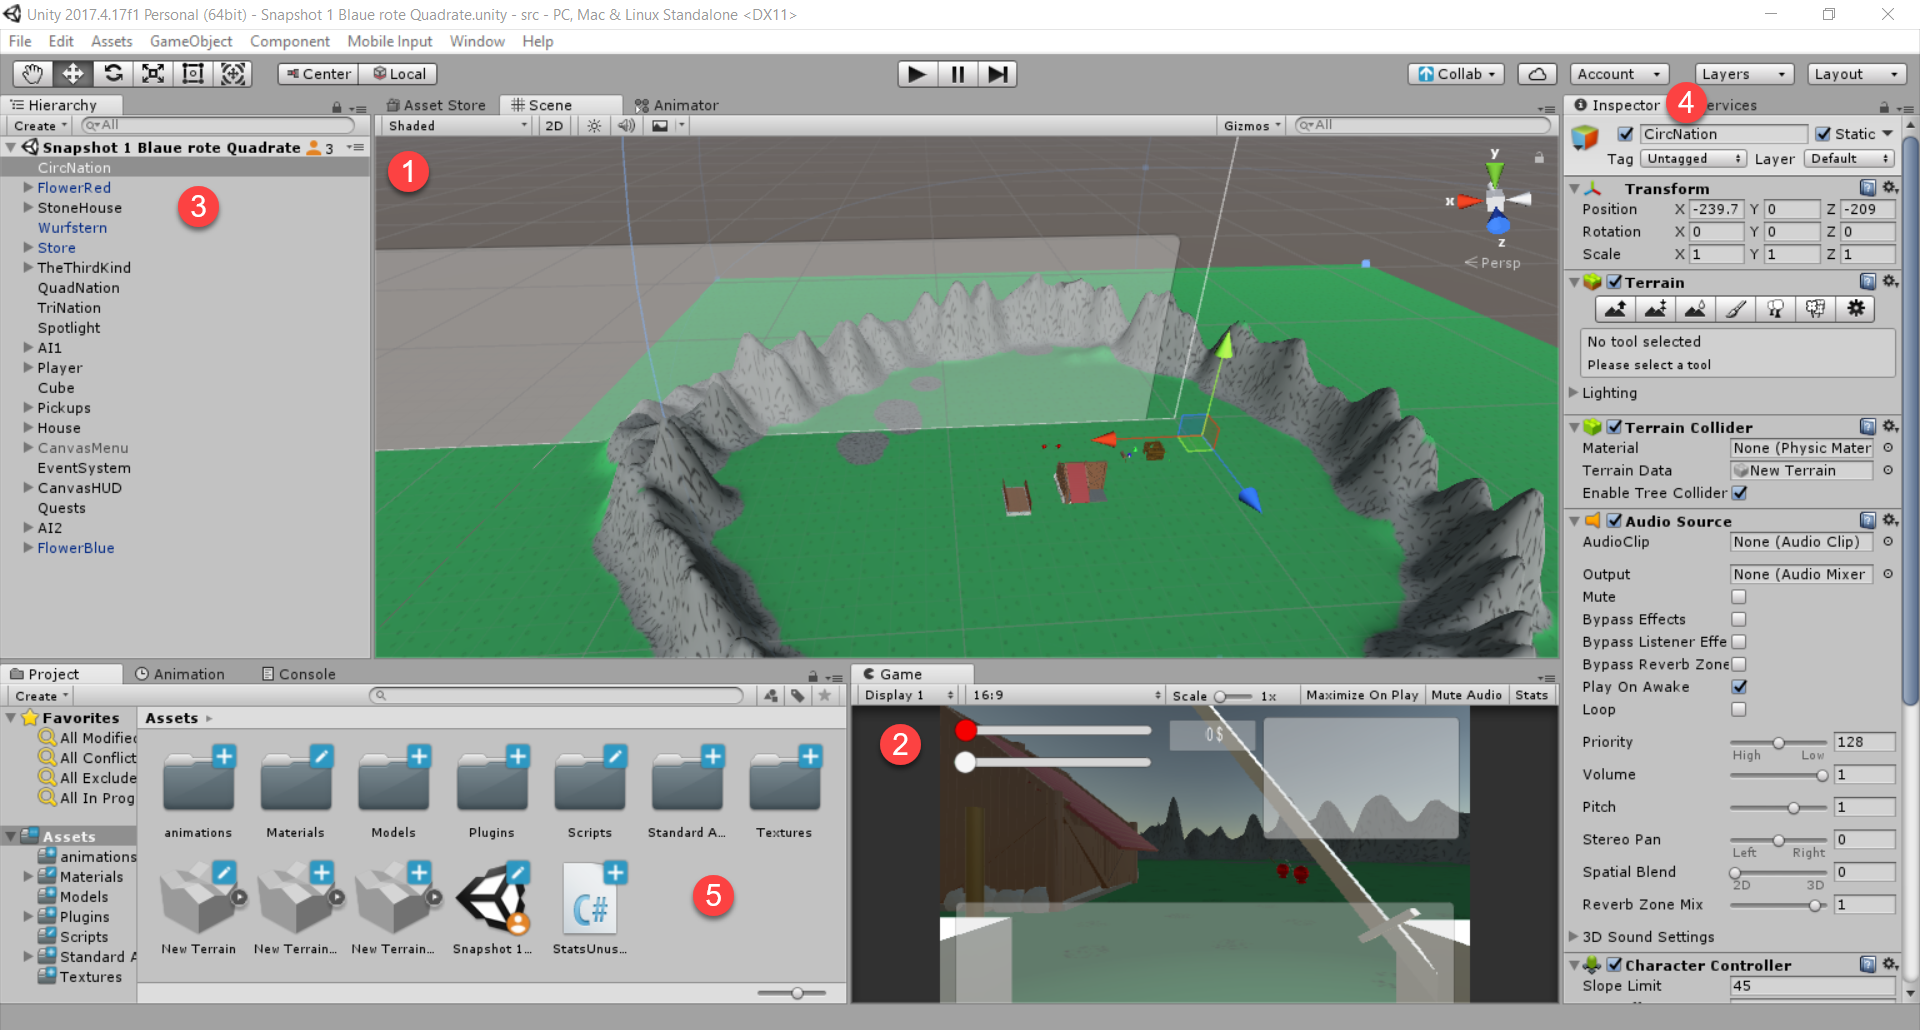
\includegraphics[scale=0.4]{screenshots/unityide.png}
\caption{Unity Benutzeroberfläche}
\end{figure}

\paragraph{Scene View (1)}
Dieses Fenster ermöglicht das Interaktive bearbeiten von Szenen und Welten.
Man kann sich in der Spielwelt überall hin und durch alle Objekte bewegen. Um Objekte zu editieren kann man sie mit X,Y und Z Achsen positionieren,
skalieren und drehen.

\paragraph{Game View (2)}
Dieses Fenster zeigt eine Vorschau des Spiels.
Sobald Play gedrückt wird, kann man darin das Spiel spielen.
Um Veränderungen auszutesten, kann man während des Spiels pausieren, Veränderungen vornehmen und das Spiel mit diesen Veränderungen fortsetzen. Sobald der Spielvorgang durch ein zweites betätigen des Play Buttons gestoppt wird, werden die Veränderungen wieder rückgängig gemacht.

\paragraph{Hierarchy (3)}
Dieses Fenster zeigt alle in der aktuell geöffneten Szene existierenden Objekte und deren Hierarchiestruktur.

\paragraph{Inspector (4)}
Dieses Fenster zeigt alle öffentlichen Parameter und Komponenten des aktuell ausgewählten Objekts (GameObject) an.

\paragraph{Project Browser (5)}
Dieses Fenster dient der visualisierten Navigation durch die Projektdateien \textbf{(Assets)}.
Alternativ wird in diesem Bereich die Konsole angezeigt, ein Fenster mit allen Outputs, Warnungen und Fehlermeldungen.

\subsection{Blender}
Blender ist eine frei verfügbare 3D Modellierungssoftware.
3D Modelle lassen sich damit viel besser und genauer bearbeiten als mit dem Standard Unity Editor. 
Zum Beispiel wäre das Erstellen einer komplexen Blüte in Unity ohne sehr grossen Zeitaufwand nicht möglich gewesen.

\begin{figure}[H]
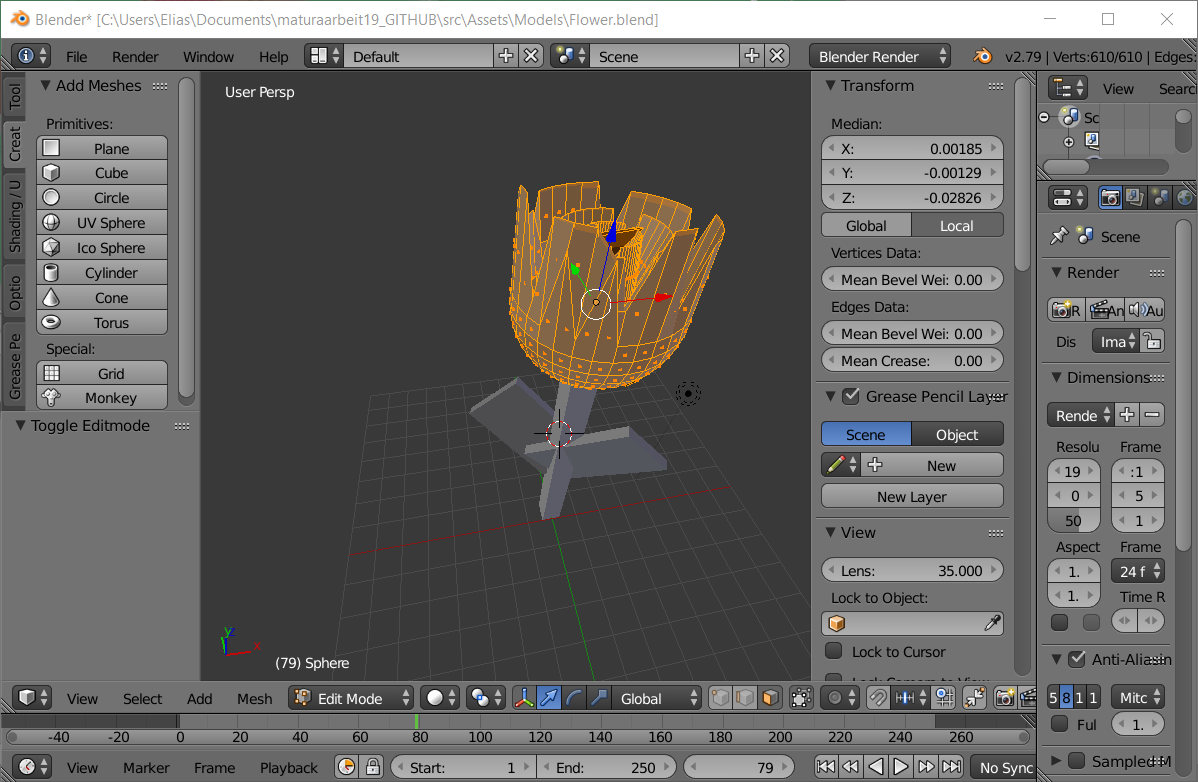
\includegraphics[scale=0.66]{screenshots/blenderflower.png}
\caption{3D Modell der Blume in Blender}
\end{figure}

\subsection{LaTeX}

Gemäss Vorgabe verfasste ich den schriftlichen Teil der Arbeit in LaTeX.
Als Editor verwendete ich Texmaker.

\subsection{MonoDevelop}

Scripts wurden in \textbf{MonoDevelop} entwickelt.
Diese Umgebung verfügt über einen hochwertigen Debugger, welcher die Fehlersuche zur Laufzeit stark erleichtert.

\begin{figure}[H]
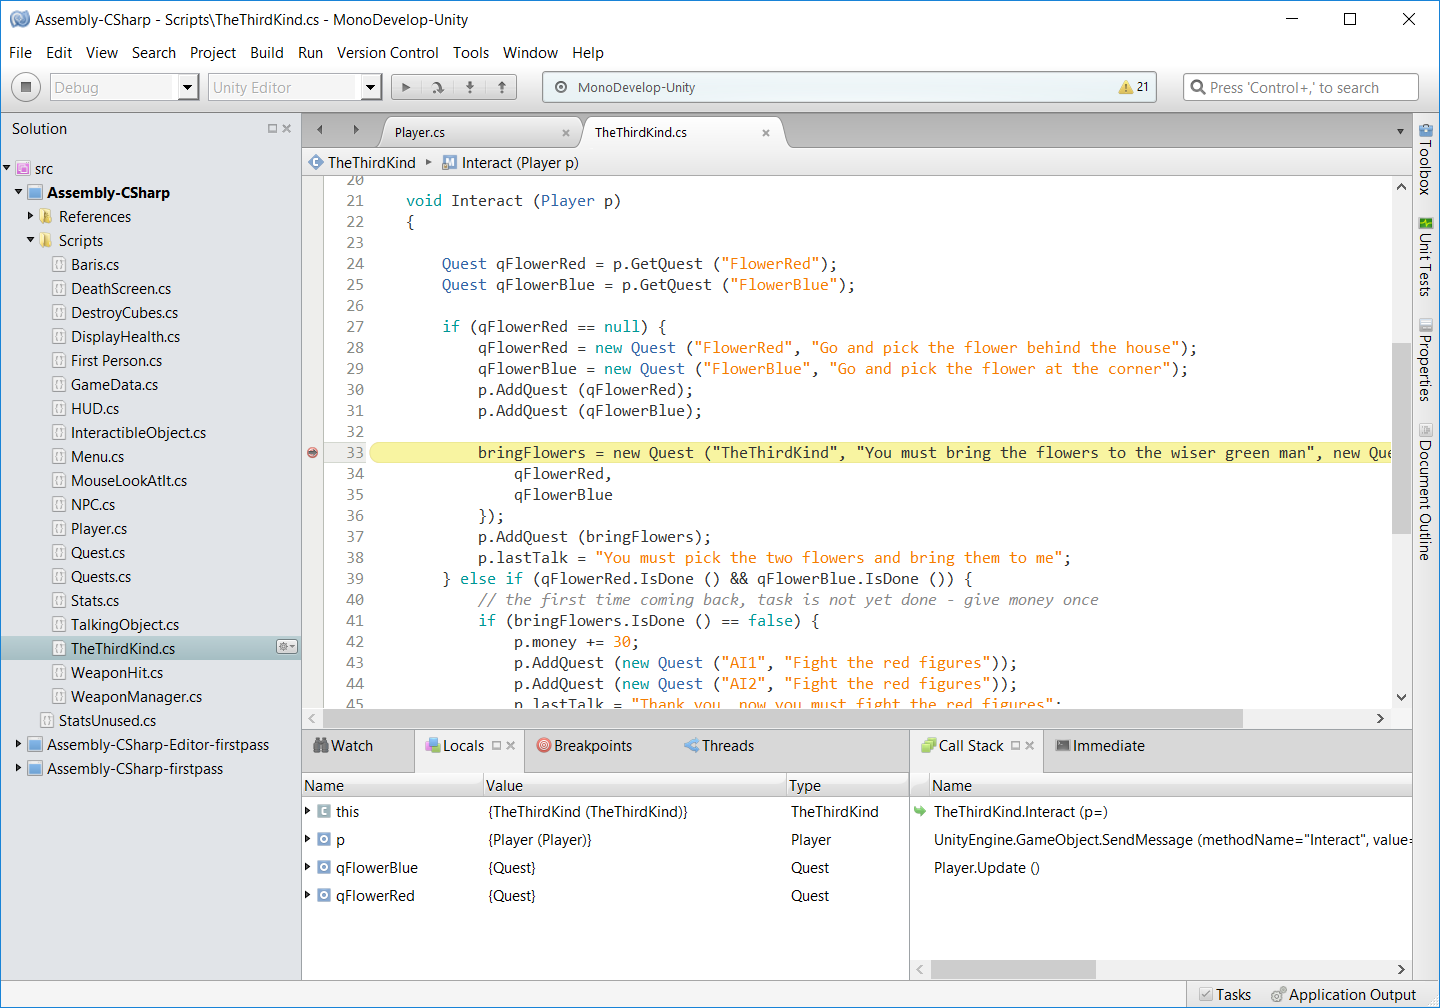
\includegraphics[scale=0.5]{screenshots/monodevelop.png}
\caption{Breakpoint im MonoDevelop Debugger mit Anzeige der Variablen}
\end{figure}

\subsection{Git}

Für die Versionsverwaltung verwendete ich das weitverbreitete Programm Git.
Als Oberfläche kam Sourcetree zum Einsatz.
Dafür erstellte ich mir einen Studentzugang auf Github.
Damit wurde die Kommunikation und das schnelle Austauschen mit meiner Betreuungsperson einfacher, da man sich nicht mehr für alles treffen musste.

\subsection{astah UML}

UML Diagramme zeichnete ich mit der gratis Studentenversion von astah UML.

\section{Programmiersprache und Framework}

\subsection{C\#}
C\# ist eine objektorientierte Programmiersprache die von Microsoft entwickelt wurde.
Unity Funktioniert mit C\# und Javascript.
Letzteres kannte ich schon, also habe ich die neue gewählt, um mein Basiswissen der Informatik zu vergrössern.


\subsection{Unity Framework}
Die Funktionalitäten (Klassen, Skripts etc.) bauen auf dem von Unity für nicht kommerzielle Zwecke gratis zur Verfügung gestellten Framework auf.
Unten sind die zwei meist benutzten Basisklassen aufgeführt.

\subsubsection{Wichtigste Basisklassen}

\paragraph{GameObject}
GameObject ist die Basisklasse für alle Objekte, die auf der Benutzeroberfläche erstellt werden.
Die wichtigste Eigenschaft eines GameObjects ist \lstinline{transform}.
Dieses beinhaltet die Position,Drehung und Skalierung im Raum.
\lstinline{GetComponent<Komponentenklasse>} ist die meist benutzte Methode. 
Sie liefert die Komponente z.B. das Kollisionsobjekt oder Skripts des GameObjects. 

\paragraph{MonoBehavior}

MonoBehavior ist die Basisklasse wenn ein GameObject mit einem Skript erweitert wird.
Die zwei geerbten Methoden die standardmässig überschrieben werden sind:
\lstinline{Start()} wird zu Laufzeitbeginn ein mal aufgerufen.
Es wird benutzt um Initialisierungen durchzuführen.

\lstinline{Update()} wird jedes Mal aufgerufen bevor ein neues Bild des Spiels berechnet wird. Darin werden Elemente wie Bewegungen fortlaufend aktualisiert.
\subsection{Physik}

\subsubsection{Rigidbody}
Jedes GameObject, auf welche sich Physikalische Kräfte wie Gravitation auswirken besitzt einen Rigidbody.
\begin{figure}[H]
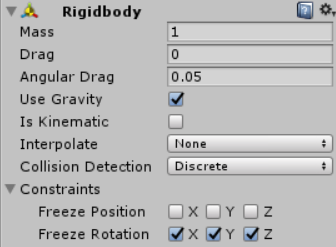
\includegraphics[scale=1]{screenshots/rigidbody.png}
\caption{Rigidbodykomponente}
\end{figure}
Hier wird die Masse des Players auf 1 festgelegt. Dies wird z.B. beim berechnen des Springens verwendet.

\subsubsection{Kollisionen}
\label{subsubsec:collider}
Die Kollisionserkennung ist einer der wichtigsten Bestandteile eines Spiels. Sie werden nicht nur für die Geltendmachung eines Treffers verwendet sondern sie entscheidet auch, wann z.B. ein Element im Sichtfeld eines Spielers ist oder nicht.
Die Hauptkomponente für das Feststellen einer Kollision ist der Collider.
Dessen Umrisse werden in der IDE definiert.
\begin{figure}[H]
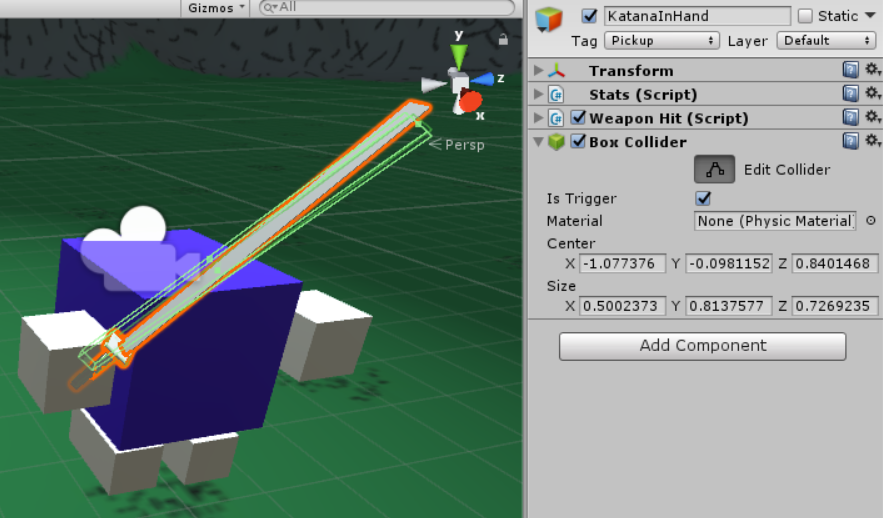
\includegraphics[scale=0.8]{screenshots/katanacollider.png}
\caption{Kollisionskomponente des Katanas}
\end{figure}
Hier sieht man den Collider in Grün. Man sieht dass er nicht die ganze Waffe abdeckt, da nur die Klinge als Trefferzone gelten soll.

Um diese Kollision einem Skript zu übermitteln gibt es zwei Methodengruppen.
OnCollision: OnColision wird ausgelöst, sobald ein Physikalischer Treffer zwischen zwei Körpern festgestellt wird.
OnTrigger: OnTrigger wird ausgelöst, wenn ein designierter Collider getroffen wird. Dieser muss hierbei nicht zwischen zwei Körpern stattfinden, sondern z.B. bei einem Treffer einer Vektorabfrage (\cref{subsubsec:interactibleobject})

\section{Glossar}

Im Folgenden möchte ich die wichtigsten Fachbegriffe kurz erläutern. \footfullcite{unity3dglossary}

\paragraph{Game-Engine}
Ein spezielles Programm, welches die grundlegende Funktionalität für den Ablauf und die Steuerung des Spieles zur Verfügung stellt.





\chapter{Prozess}

\section{Arbeitsmethodik}

Arbeitsjournal(taten:was,zeiten:wann, stunden:wie lange)
(Grafik und Code)

\subsection{Vorgehensweise} 
Ich trage jeden Tag ein Heft in meiner Schultasche mit mir, in welchem ich auftauchende Ideen sofort aufschreibe/aufzeichne.
Wenn ich dann wieder an meinem Computer sitze, werden diese Ideen nochmals durchgeschaut und entweder verworfen oder Implementiert.
Ich sorge dafür dass ich jede Woche \textbf{mindestens einmal} daran Arbeite, und höre wenn ich mal begonnen habe auch nicht so schnell wieder auf.

\subsection{Dokumentation}
Meine quellen (meistens Youtube oder Udemy Tutorials) so wie der damit verbundene Fortschritt dokumentiere ich in einem \textbf{TXT File}.
Die Versionskontrolle erfolgt über \textbf{GitHub}.

\section{Problemstellungen und deren Umsetzung}

\subsection{Allgemeine Arbeitsweise}
Nachdem ich die grundlegenden Objekte wie z.B. den Spieler und die einfachen Funktion wie z.B. Laufen erstellt hatte, ging es daran, das Spiel zu erweitern. Ich bin nicht einer der wenigen die sich ein Script im Kopf überlegen und dies dann fehlerfrei beim ersten Versuch zum laufen kriegen können. (Noch nicht).

Wenn es also an die Umsetzung einer Idee kam, schrieb ich den Code in ein schon existierendes Skript.
Falls es nicht funktionierte, wurde entweder ein anderer Ansatz gewählt oder ich arbeitete daran bis es geklappt hat.
Sobald funktional alles glatt lief, musste der Code aufgeräumt werden. Dabei wurden die noch vorhandenen Spuren der nicht erfolgreichen Versuche entfernt, der gewünschte Code allenfalls bereinigt und vereinfacht. Wenn es grosse Code-Teile waren, dann sollten die benötigten Teile eigenständig werden, denn ein einziges riesiges Skript welches das ganze Spiel steuert, ist weder besonders gut für das rasche Arbeiten, noch wird es von anderen Programmierern/Programmiererinnen gerne gesehen, da die Übersichtlichkeit verloren geht.

Das Aufräumen oder Auslagern passierte dadurch, dass ich entweder manuell ändert oder ein neues Skript erstellt habe und dort den getesteten Code hinein kopierte, oder ich habe den Code mit Hilfe von MonoDevelop \textbf{refaktorisiert} (Erklärung im übernächsten Abschnitt). 

\subsection{Inspirationsquellen}
Was das erfinden der Objekte und Geschichte angeht, diente mir vor allem meine rege Fantasie als Inspiration.
Doch ab und an half auch diese nichts, gerade dann wenn es um komplizierte Funktionalitäten 
ging (e.g. Vektoren für Interact und Jump).
%todo screenshot?
In diesen Fällen konsultierte ich eine Website namens Udemy. Diese bietet eine grosse Spannweite an Kursen. Mein Vater hatte mir dort vor ein paar Monaten einen Programmierkurs für C\# geschenkt, welcher sich nun als nützlich erweisen sollte.
Dieser Kurs war eine auf sich aufbauende Videoserie, in welcher ein 2D Spiel von A-Z entwickelt wurde.
Da mein Spiel jedoch 3D sein sollte und der Udemy Kurs beim besten willen nicht alle Thematiken abdecken konnte, blieb mir als oft letzte Hoffnung noch die öffentliche Tutorialwebseite von Unity. \footfullcite{unity3dtutorial}

\subsection{Refaktorisierung}
\label{subsubsec:refactoring}
Quellen in https://de.wikipedia.org/wiki/Refactoring
Umsetzung mit MonoDevelop
\paragraph{Umbennen}\mbox{} \\
Viel Refactoring, 
- Problem bei Klassennamen -> Scriptname, IDE zieht nicht automatisch mit

\paragraph{Vereinfachen}\mbox{} \\
- Mehrfach vorkommender Ausdruck, wie z.B. GetComponent<Player>... wird in eine Variable genommen

\paragraph{Aufteilen}\mbox{} \\
- eigene Klasse, WeaponManager

das Spiel: 
	zu jedem "wichtigen" GameObject:
	modell, verwendungszweck, scripts, 				schwierigkeiten

\subsection{Spielführung}
Damit das Spiel wirklich gut benutzbar wird, benötigt es gewisse Funktionen, die den Spieler unterstützen und an der Hand durch das Spiel begleiten:
\begin{itemize}
\item Um nicht jedes mal neu anfangen zu müssen, gibt es ein Menü mit der Möglichkeit des Unterbruchs und Wiederaufnahmedes Spiels, verbunden mit einer Speicherfunktion des Spielstands.
\item Das Heads-Up-Displays (HUD) hat die Aufgabe, dem Spieler alle nötigen Informationen über den Zustand seiner Spielfigur zu liefern.
\end{itemize}



\subsubsection{Menu}
Skript: Menu.cs\\
Start Menu

\begin{figure}[H]
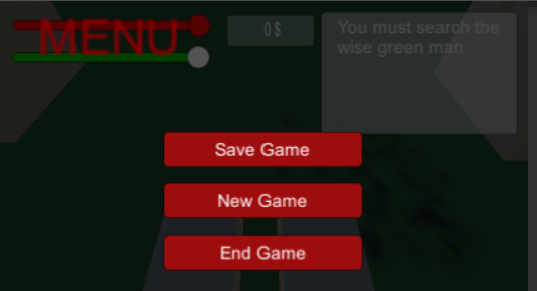
\includegraphics[scale=1]{screenshots/menuscreen.png}
\caption{Menü}
\end{figure}

Das Menü beinhaltet vier Elemente: Einen \textbf{Canvas}, also eine "Plache", die für uns hier als Hintergrundabdunklung fungiert.
Dann gibt es 3 Buttons:
\paragraph{new game}
Dies setzt alle im Savefile gespeicherten daten zurück und Startet das Spiel neu.

\begin{lstlisting}
//Starts a new game
public void OnButtonNewPressed ()
{
	print ("Write some code here");
	player.gameData.InitNewGame ();
}

\end{lstlisting}

\paragraph{save game}
Dieser Knopf tut nichts anderes als bestimmte Daten wie die X,Y,Z position des Spielers in ein Textfile zu schreiben. Bei einem Neustart des Spiels werden diese Angaben wieder eingelesen und  übernommen.

\begin{lstlisting}
//Speicherfunktion
public void OnButtonSavePressed ()
{
	Debug.Log ("Speichern");
	player.gameData.SaveGame ();
}
	
\end{lstlisting}

\paragraph{end game}
Das einzige, was dieser Knopf macht, ist einen Unity Befehl namens \lstinline{Application.quit}  ausführen, welcher das ganze Programm beendet. 

\begin{lstlisting}
//Ends game
public void OnButtonEndPressed ()
{
	Debug.Log ("Spiel Beendet");
	Application.Quit ();
}
\end{lstlisting}

\subsubsection{GameData}
Skript: GameData.cs
Die Daten des aktuellen Spiels
- Stand speichern
\\


\subsubsection{Heads-Up Display HUD}
Skript: HUD.cs
Heads-Up Display

\begin{figure}[H]
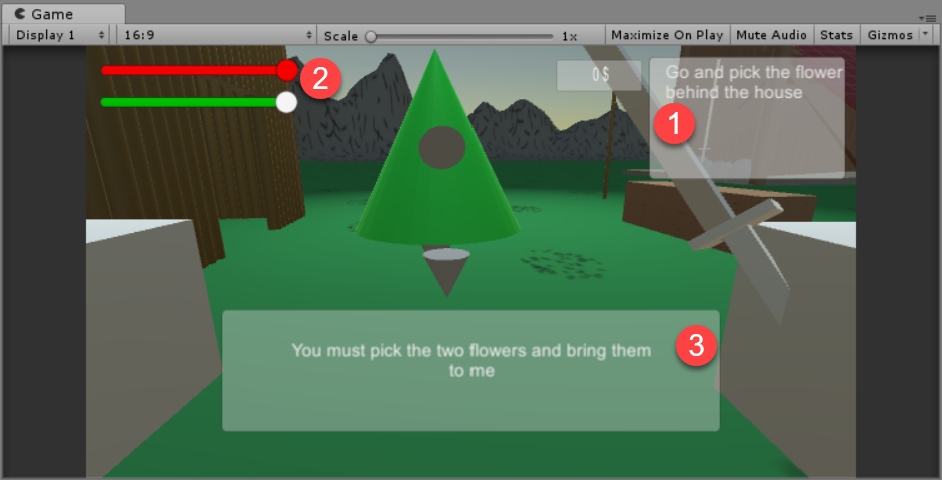
\includegraphics[scale=0.8]{screenshots/hud.png}
\caption{HUD}
\end{figure}

Ein Heads-up Display ist eine Anzeigefläche die sich nicht aus dem Sichtfeld bewegt, auch wenn der Benutzer seinen Kopf neigt und oder schwenkt.
Somit sind die Informationen in jeder situation Ablesbar.
 
\paragraph{Aufgabenbereich (1)}\mbox{} \\
Der Aufgabenbereich befindet sich oben rechts.
Darin wird die jeweils aktuelle Aufgabe angezeigt.

\paragraph{Zustandsdisplay (2)}\mbox{} \\
Das Zustandsdisplay befindet sich oben links im HUD.

Es besteht aus zwei Schiebereglern \lstinline{Slider}, einer für die Gesundheit \lstinline{player.health} und einer für die Ausdauer \lstinline{player.stamina} des Spielers.
Ein Schieberegler ist ein 2D Balken, der einen Wert verkörpert. Man kann ihm in der Entwicklungsumgebung einen minimalen und einen maximalen Wert geben, hier ist das bei beiden 0-100.

\begin{figure}[H]
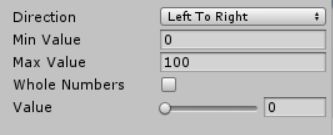
\includegraphics[scale=1]{screenshots/nullhundert.png}
\caption{Slider value}
\end{figure}

Abgefüllt werden diese Balken durch das HUD-script, welches bei jedem \lstinline{Update} Aufrug die aktuellen Werte aus dem \lstinline{Player} Objekt ausliest und in die Schieberegler weitergibt.

\begin{lstlisting}[caption={Schieberegler erstellen}]
public class HUD : MonoBehaviour
{
	(...)
	// Gesundheit Schieberegler
	private Slider healthSlider;
	// Ausdauer Schieberegler
	private Slider staminaSlider;
	(...)
	// Statusinformationen aus Spieler übernehmen und anzeigen
	void Update()
	{
		(...)
		healthSlider.value = player.health;
		staminaSlider.value = player.stamina;
		(...)
	}
}
\end{lstlisting}

\paragraph{Kommunikationsbereich (3)}\mbox{} \\
Der Kommunikationsbereich befindet sich zwischen der Mitte und dem unteren Drittel des Bildschirmes.
Normalerweise ist er deaktiviert.
Aktiviert wird er dann, wenn ein \lstinline{Interact} Aufruf das Attribut \lstinline{lastTalk} des Players neu setzt:

\begin{lstlisting}[caption={Kommunikation setzen}]
void Interact(Player p)
{
	(...)
	p.lastTalk = "You must pick the two flowers ...";
	(...)
}
\end{lstlisting}

Im folgenden Codeausschnitt wird gezeigt, wie das ein und ausschalten der Sprechblase und  das aktualisieren des beinhalteten Textes funktioniert. Dies geschieht in der periodisch aufgerufenen \lstinline{Update} Methode, \lstinline{Time.time} liefert die Zeit in Sekunden seit Spielstart.

\begin{lstlisting}[caption={Sprechblase ein- und ausblenden}]
public class HUD : MonoBehaviour
{
	// Die Spielerinstanz, welche alle Informationen liefert
	public Player player;

	// Feld, welches die Sprechblase beinhaltet
	private GameObject talking;
	// Textobjekt, welches den gesprochenem Text anzeigt
	private Text talkingText;
	// Zeitpunkt, als die letzte Blase angezeigt wurde, 0 wenn keine 
	// angezeigt wird
	private int speechDisplayedTime = 0;
	// Darstellungszeit der Sprechblase
	private const int speechDisplayDuration = 15;

	(...)
	
	// Update wird pro frame einmal aufgerufen
	// Statusinformationen aus Spieler übernehmen und anzeigen
	void Update()
	{
		(...)
		string lastTalk = player.lastTalk;
		// wenn mit dem Spieler seit letztem Mal gesprochen wurde
		if (lastTalk.Length > 0) {
			// anzeigen der Sprechblase
			player.lastTalk = "";
			talking.SetActive(true);//hier wird die Sprechblase aktiviert
			talkingText.text = lastTalk;
			// Zeitpunkt des Anzeigens merken
			speechDisplayedTime = (int)Time.time;
		} else {
			// kein neuer text, überprüfe ob die Sprechblase 
			// wieder versteckt werden soll
			if (speechDisplayedTime > 0) {
				if ((int)Time.time - speechDisplayedTime > 
					speechDisplayDuration) {
					speechDisplayedTime = 0;
					talking.SetActive(false);//hier wird die Sprechblase deaktiviert
					talkingText.text = "";
				}
			}
		}	
	}
}
\end{lstlisting}


%todo ein ausblenden
\subsection{Spieler}

\begin{figure}[H]
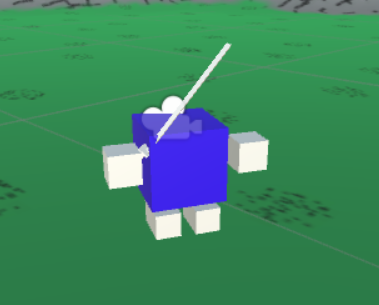
\includegraphics[scale=1]{screenshots/player.png}
\caption{Player 3D Modell}
\end{figure}

Das Modell besteht rein aus Würfeln und Rechtecken.


\subsubsection{Player}
Skript: Player.cs
Der Spieler
- bewegen
- kämpfen
- health

\paragraph{Gesundheitszustand}\mbox{} \\
Der Gesundheitszustand wird im HUD angezeigt und kann über einen Methodenaufruf z.B. von Waffen verändert werden.

Der Player wie auch der NPC haben beide in ihrem eigenen Script das Setup ihrer Gesundheit.
\begin{lstlisting}
//Health
public float health = 100f;
\end{lstlisting}
Um die Gesundheit zu verändern benutze ich eine Methode, in der der Wert um den die Gesundheit geändert werden soll in den Aufruf mitgegeben wird. Dieser Wert kann sowohl positiv als auch negativ sein.
Dieser Wert wird dann zur vorherigen Gesundheit addiert.


Dass die Gesundheit nicht über 100 geht und falls sie unter 0 geht man auch tatsächlich stirbt, dafür sorgen die If-statements. Für den NPC sieht es so gut wie gleich aus.
\begin{lstlisting}
public void ChangeHealth(float change)
{
	health += change;

	if (health > 100.0f)
		health = 100.0f;
	else if (health < 0.0f) {
		Debug.Log("YOU ARE DEAD");
		model.SetActive(false);//lässt das gameObject verschwinden
	}
}
\end{lstlisting}
OO-Beispiel:Data Encapsulation, Single Definition Rule, private members, public Methods, , damit keine Veränderung von aussen, und 1 Ort, an welchem z.B. Entscheide über Tod gefällt werden können.

\subsubsection{MouseLookAtIt.cs}
Skript: MouseLookAtIt.cs\\
Drehe Spieler mit der Maus

OO-Beispiel:Composition/Delegation vom Player aus

\subsection{Animationen}
In Unity Animationen zu erstellen braucht weniger Geschick als Geduld.
Jede der drei Spezies hat drei Animationen.


\subsubsection{Die verschiedenen Animationen}
\paragraph{Lauf-Animation}
%Todo screenshots

Die Lauf-Animation besteht daraus, dass der Fuss gehoben nach forne geht und gesenkt nach hinten. Diese Animation wird versetzt auf den zweiten Fuss so versetzt kopiert, dass immer wenn der eine Fuss hinten ist ,der andere forne ist und umgekehrt.

Die grösste Schwierigkeit bei dieser Animation war es, die beiden Füsse auf einander abzustimmen.
Dazu kam, dass die Fortbewegungsgeschwindigkeit des Objekts ungefähr mit der Fussbewegung der Animation übereinstimmen sollte.
%todo Player walkanimation
%Todo NPC walkanimation

TheThirdKind hat zwar eine Laufanimation, Benutzt sie jedoch nicht.
%Todo T3K walkanimation
\paragraph{Untätig-Animation}
Die Untätig-Animation oder auch \textbf{Idle-Animation} war die einfachste Animation zum erstellen, da sie rein aus einem synchronen heben und senken der Hände besteht.

\paragraph{Angriffs-Animation}

Diese Animation war die schwierigste, da sie neben einer Positionsveränderung auch eine Drehung verlangte.
Das Problem war, dass bei einer Drehung der Hand diese aus ihrer Form fiel und die in der Hand gehaltene Waffe ebenso falsch skaliert wurde.

Dieses Problem behob ich mit Feintuning and den Kurven.
Das bedeutet es verändert sich immer noch ein wenig, aber nicht mehr in einem störenden Ausmass.

\subsubsection{Animation}
Um eine Animation zu erstellen gibt man ihr zuerst einen Namen.
Danach öffnet sich ein leeres Fenster des Unity-Animators.
Dort hinein kann man per drag and drop GameObjekte hinzufügen und wählen, ob man Rotation, Proportion oder Position verändern will (es gibt noch viele andere Optionen die man verändern 
kann, aber diese habe ich nicht benutzt).

\begin{figure}[H]
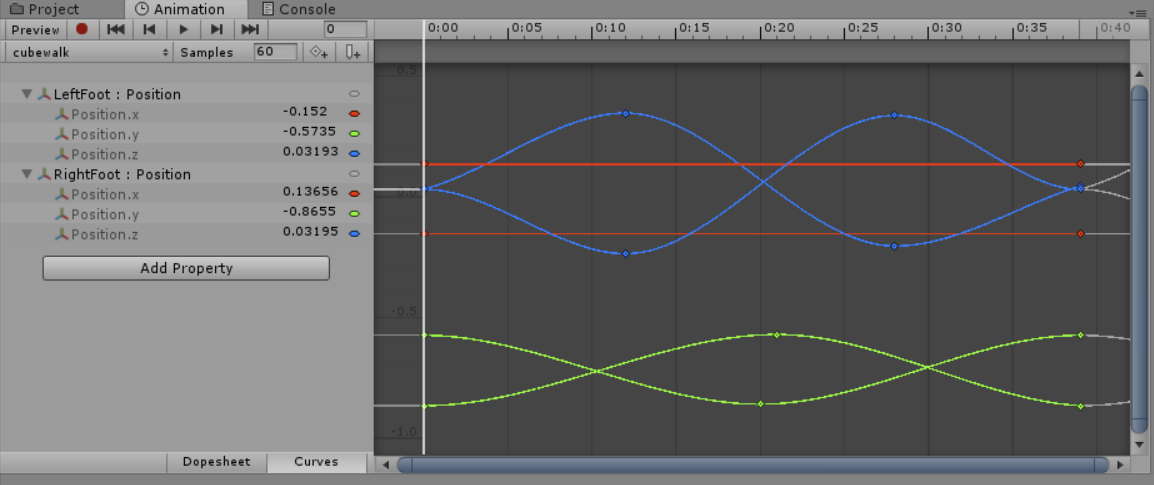
\includegraphics[scale=0.7]{screenshots/animations.png}
\caption{Animationskurven}
\end{figure}

In diesem Beispiel handelt sich hier um eine Laufanimation welche nur die Füsse kontrolliert.
Man sieht hier besonders, wie sich die Füsse nicht Ruckartig, sondern fliessend und einander entgegengesetzt bewegen.

\subsubsection{Animator}
Der Animator ist das Element, welches den Wechsel zwischen verschiedenen Animationen übernimmt.
Zeiger können von einem Zustand auf einen anderen verweisen.
Diese Zeiger wiederum kann man an Bedingungen koppeln.
\begin{figure}[H]
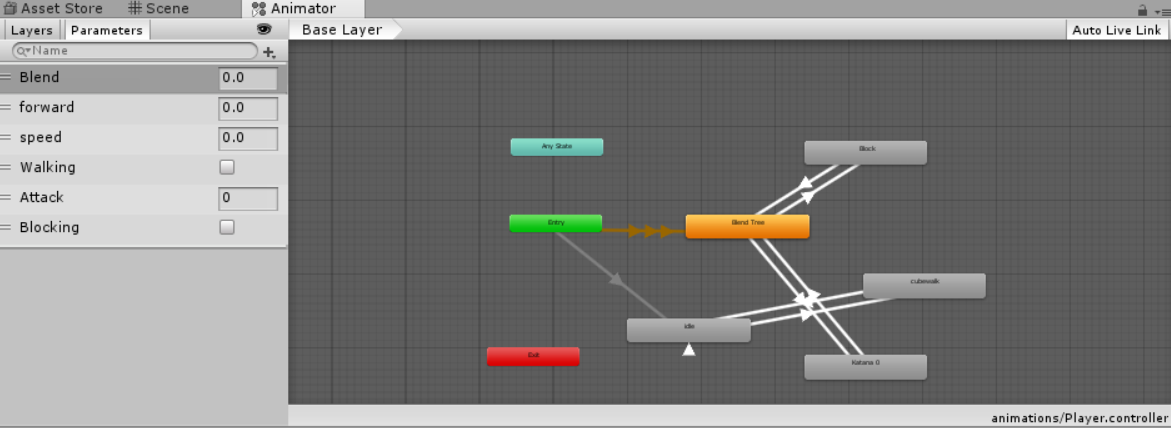
\includegraphics[scale=0.7]{screenshots/animator.png}
\caption{Animator}
\end{figure}

%todo: UML für zustandsübergänge?

\subsection{Waffen}
%todo shuriken?

Es gibt drei  Waffen: Das Katana, Das Bo, und die Fäuste.
Jede Waffe hat verschiedene Werte was Schaden, Ausdauerkosten und Reichweite angeht.
\begin{figure}[H]
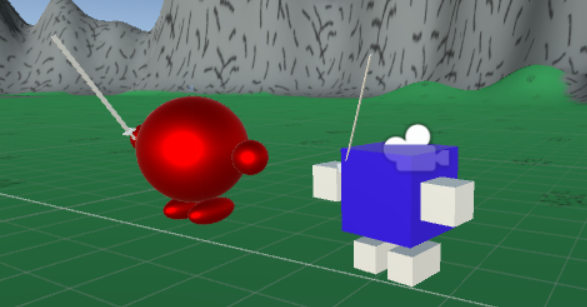
\includegraphics[scale=1]{screenshots/katana.png}
\caption{Katana}
\end{figure}

\begin{figure}[H]
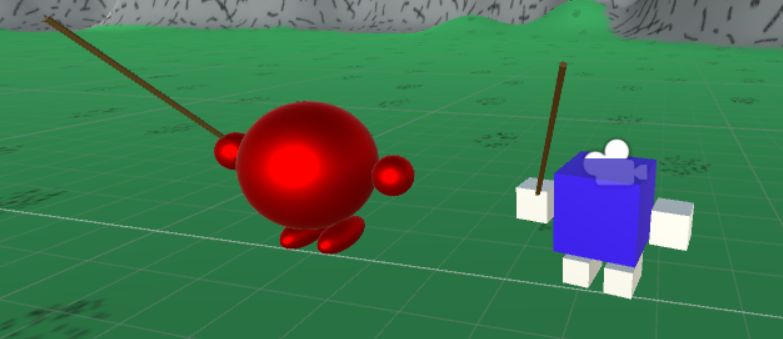
\includegraphics[scale=1]{screenshots/bo.png}
\caption{Bo}
\end{figure}



\subsubsection{Stats}
Skript: Stats.cs\\
Werte der Waffen, verwendet von WeaponHit

\begin{lstlisting}
public string WeaponName = "Katana";
public float WeaponDamage = 35;
public float WeaponDefense = 15;
public float WeaponRange =	3;
public float WeaponSpeed = 3;
public float WeaponStamina = 10;
\end{lstlisting}


\subsubsection{WeaponHit}
Skript: WeaponHit.cs\\

Jede Waffe hat einen \lstinline{Collider} (siehe \cref{subsubsec:collider}). Dieses Element löst ein Ereignis \lstinline{OnTriggerEnter} Ereignis aus, sobald es mit einem anderen \lstinline{Collider} in Berührung kommt.
Das hier verwendete Script ermittelt das Kennzeichen des getroffenen Objekts und fügt Schaden zu, entweder dem Gegner oder dem Spieler selbst, je nachdem ob es sich dabei um ein Element mit dem Tag "Enemy" oder mit dem Tag "Player" handelt.
Der Wert des Schadens, berechnet sich aus der Waffenwirkung, welche es aus den \lstinline{Stats} der jeweiligen Waffe ausliest.

\begin{lstlisting}[caption={Waffentreffer}]
damage = Self.GetComponent<Stats>().WeaponDamage;

void OnTriggerEnter(Collider col)
{
	if (col.tag == "Enemy") {
		GameObject.Find (col.name).GetComponent<NPC>().ChangeHealth(-damage);
		Debug.Log(damage + " Damage applied to " + col.name);
	} else if (col.name == "Player") {
		GameObject.Find (col.name).GetComponent<Player>().ChangeHealth(-damage);
		Debug.Log(damage + " Damage applied to " + col.name);
	}
}
\end{lstlisting}

\paragraph{kämpfen}\mbox{} \\
- damage

\subsubsection{WeaponManager.cs}
Skript: WeaponManager.cs
Verwaltet die verschiedenen Waffen und deren Einsatz
- Waffen wechseln
- animation

\subsection{Figuren}


\subsubsection{InteractibleObject}
Skript: InteractibleObject.cs
Alle Drittobjekte mit denen interagiert werden kann

Die Funktion des interagierens sendet einen Strahl aus.
Wenn dieser Strahl etwas trifft wird überprüft, ob das getroffene GameObject den Tag "Interactive" hat. Falls ja, wird eine Nachricht mit dem Inhalt "Interact" an das getroffene Objekt geschickt. Falls der Tag nicht vorhanden ist, passiert nichts.

\begin{lstlisting}[caption={Auslösen der Interaktion}]
// Interaktion (standard button "E")
if (Input.GetAxis ("Interact") > 0f) {
	Vector3 forward = transform.TransformDirection (Vector3.forward);

	if (Physics.Raycast (transform.position, forward, out interactHit, 10)) {	
		
		Debug.DrawLine (transform.position, interactHit.point);
		if (interactHit.collider.gameObject.tag == "Interactive") {
			// send a message
			interactHit.collider.gameObject.SendMessage ("Interact", (Player)this);
			// update quest - if existed
			quests.Interacted(interactHit.collider.gameObject);
		}
	}	
}
\end{lstlisting}

\paragraph{Sammeln}\mbox{} \\
Wie jedes gute RPG braucht auch das meine eine klassische Sammel-Aufgabe.
Normalerweise schicken einen diese Aufgaben über die gesamte Karte um eine gewisse Anzahl an Gegenständen zu sammeln.
In diesem Spiel ist der Weg nicht allzu weit: sie stehen direkt hinter dem Haus der Figur, die einem den Auftrag gibt.

Sobald der Spieler mit den Blumen interagiert, verschwinden sie: sie wurden gepflückt.
Dies passiert, weil die oben beschriebene Nachricht \lstinline{Interact} bei dem Objekt \lstinline{Blume} ein Skript ausführt, welches das Objekt deaktiviert.
\begin{lstlisting}[caption={Standardimplementation von Interact}]
void Interact(Player p)
{
	gameObject.SetActive(false);
}
\end{lstlisting}
 
\paragraph{Reden}\mbox{} \\
Es gibt nur ein einziges \lstinline{GameObject} das mit dem Player redet, und das ist \lstinline{TheThirdKind}.
 Das Gesprochene erscheint in einer Sprechblase.
 
\begin{lstlisting}[caption={Gesprochenes aktualisieren}]
void Update()
{
	(...)
	string lastTalk = player.lastTalk;
	// wenn mit dem Spieler seit letztem Mal gesprochen wurde
	if (lastTalk.Length > 0) {
		// anzeigen der Sprechblase
		player.lastTalk = "";
		talking.SetActive(true);
		talkingText.text = lastTalk; //hier wird der Text ersetzt
		// Zeitpunkt des Anzeigens merken
		speechDisplayedTime = (int)Time.time;
	} 
}
\end{lstlisting}
Um dies auszulösen, muss \lstinline{lastTalk} des Spielers geändert werden.
Dies passiert, wenn der Spieler mit dem \lstinline{TheThirdKind} Objekt Interagiert 
\begin{lstlisting}
void Interact(Player p)
{
	p.lastTalk = "You must pick the two flowers and bring them to me";
}
\end{lstlisting}


OO-Beispiel: Subclassing, Polymorphism

\subsubsection{NPC.cs}
Skript: NPC.cs
Autonome Gegner
\begin{figure}[H]
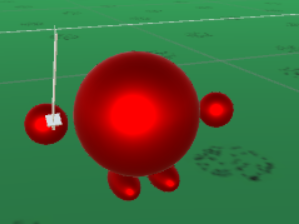
\includegraphics[scale=1]{screenshots/npc.png}
\caption{NPC 3D Modell}
\end{figure}
Das 3D Modell besteht rein aus Kugeln.

\paragraph{aktivieren}
Dass der NPC auf den Spieler aufmerksam wird, muss er ihn zuerst sehen.
Dafür hat der NPC einen Collider, welcher sein Sichtfeld darstellt.
\begin{figure}[H]
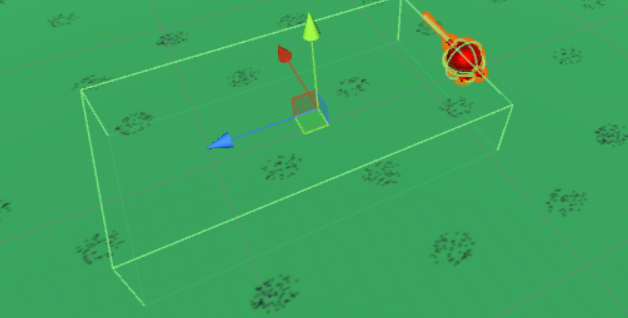
\includegraphics[scale=1]{screenshots/fov.png}
\caption{Sichtfeld des NPCs}
\end{figure}
Sobald der Spieler diesen Collider einmal berührt hat, wird der Bewegungscode aktiviert.
\begin{lstlisting}
public bool hasseenplayer = false;
private void Start()
{
	player = GameObject.FindGameObjectWithTag ("Player");
}
	
//Spotting player
void OnTriggerEnter(Collider fov)
{	
	if (fov.name == "Player") {
		Debug.Log("has seen");
		hasseenplayer = true;
	}
}
\end{lstlisting}
\paragraph{bewegen }
Der NPC richtet sich nach dem Spieler aus und geht so lange auf ihn zu, bis die X und Y Koordinaten auf eine Differenz von 1 genau übereinstimmen.
Dann Spielt der NPC seine attackier-Animation ab.
\begin{lstlisting}
if (hasseenplayer == true) {	
	//if player is in range, attack (set fighting true)
	Vector3 forward = transform.TransformDirection (Vector3.forward);

	//check if "player" is in Range to attack, if so do so
	if (Physics.Raycast (transform.position, forward, out hit, 10)) {	

		Debug.DrawLine (transform.position, hit.point);
		if (hit.collider.gameObject.tag == "Player") {
			fighting = true;
			Debug.Log("NPC is attacking");
		} else {
			fighting = false;
			anim.ResetTrigger ("Attack");
		}

		//if fight is true fight,
		if (fighting == true) {
			anim.SetTrigger ("Attack");
			//fight
		} else {	
			anim.SetBool ("iswalking", true);
					
			if (player.transform.position.x > (transform.position.x - 1)) {
				//go right
				transform.position += new Vector3 (Speed * Time.deltaTime, 0, 0);
            		
			} else {
				//Go left
				transform.position -= new Vector3 (Speed * Time.deltaTime, 0, 0);
					}
			//go towards Players'z
			if (player.transform.position.z > transform.position.z) {
				//Go up
				transform.position += new Vector3 (0, 0, Speed * Time.deltaTime);
			} else {
				//go down
				transform.position -= new Vector3 (0, 0, Speed * Time.deltaTime);
			}
			transform.LookAt (target);//https://docs.unity3d.com/ScriptReference/Transform.LookAt.html
		}
	} else {
			anim.SetBool ("iswalking", false);
	}
}

\end{lstlisting}
\subsubsection{TheThirdKind.cs}
Skript: TheThirdKind.cs
Weiser der den Spieler über die nächsten Schritte

TheThirdKind ist ein Schlüsselelement des Spiels. Zu ihm muss man zu Beginn gehen, um die Blumen-Aufgabe zu erhalten.
Er sollte der aus vielen RPGs bekannten Auftraggeber sein, der einen quer durch die Welt schickt um ein paar Rohstoffe zu sammeln.
\begin{figure}[H]
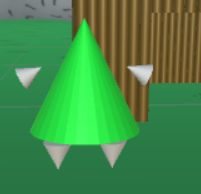
\includegraphics[scale=1]{screenshots/t3k.png}
\caption{ TheThirdKind 3D Modell}
\end{figure}
Dieses 3D Modell besteht nur aus Kegel.

\subsection{Aufgaben}

\subsubsection{Quest.cs}
Skript: Quest.cs
Eine einzelne Aufgabe

\subsubsection{Quests.cs}
Skript: Quests.cs
Die Sammlung aller Aufgaben
- Hinzufügen
- Kontrollieren

\begin{itemize}
\item Grundgerüst (Einfaches Terrain, Lightsource, charactermodel+controller) //Implementiert
\item Waffensystem	//currently working on
\item Player HUD
\item Inventarsystem
\item NPCs
\item Skilltree
\item Savegames
\item Story
\item Quests

\end{itemize}



%%%

OO

Subclasses

Composition

Delegation

Shielding Interface

Encapsulation and Information Hiding

%%%

\section{Versionsverwaltung}

% https://forum.unity.com/threads/solved-missing-prefabs-with-freshly-downloaded-project-windows.411721/

Blender muss installiert sein, sonst kann das Projekt von Unity nicht geöffnet werden.

\section{Verteilung und Test}

\subsection{Verteilung über Github}

Da ich von Anfang an die Versionskontrolle dieser Maturarbeit mit Github bewältigt habe konnte sich theoretisch jeder der meinen Github-Namen kannte meine komplette Arbeit herunterladen.\cite{csomormaturaarbeit19github}
Ich erzählte also in der Schulklasse von meinem Projekt und einige meiner Freunde fragten, ob sie es downloaden könnten.

Leider schieden sofort einige Kandidaten aus, welche kein Windows-Gerät besassen.
Aus den restlichen drei Interessierten entstanden die SimpleRPG-Beta-Tester.

\subsection{Testphase}

Diese informierten mich schon früh über Abstürze, Bugs und Glitches.
An ihnen konnte ich ebenfalls die Effektivität meines \textbf{README.TXT} files zu testen, welches ihnen Instruktionen für das korrekte aufstarten des Spiels und Informationen über die Steuerung lieferte.
Oft redeten wir in den kurzen Pausen zwischen den Lektionen über mein Spiel.
Das gab mir eine Plattform wo ich meine weiterführenden Ideen präsentieren und sofort Feedback einholen konnte, was mir half, mich auf Inhalte zu fokussieren, die von der Mehrheit gemocht wurde.




\chapter{Resultate}

\section{Erkenntnisse}
Meine grösste Erkenntnis war, wie schwierig das Abschätzen von Zeiten für Programmierarbeiten ist.

Beim Programmieren ist es anders als beim schreiben eines Buches wo man sich vornehmen kann, an einem Tag eine bestimmte Anzahl an Seiten zu schreiben, so dass man bis zum Ende der Frist genug Seiten hat.
Der Aufwand für ein einzelnes Problem kann spontan zehn mal höher ausfallen als geplant. Anders herum habe ich auch einige Features viel schneller erledigt als ich es geplant hatte.

Um diesem nicht planbaren Faktor entgegen zu wirken entschied ich mich dazu, die Code-arbeiten vorzuziehen.
Dieses Vorgehen hat nun dazu geführt dass ich sehr guten Code habe, aber leider weniger Spielinhalt als ich es mir wünschte.

Beim Lösen eines Problems war einer meiner besten Ansprechpartner das Internet.
Leider gibt dieses nicht nur eine Antwort auf eine Frage, sondern ich bekomme 100 Antworten von welchen 80 ähnliche Probleme haben, aber nur 20 das gleiche.
Von diesen 20 bekomme ich dann 3-6 verschiedene Lösungsvorschläge und muss ausprobieren, welcher am besten für mein Projekt geeignet ist.




\section{Erweiterungsmöglichkeiten}
Hätte ich mehr Zeit, wären mehr Aufgaben und mehr Interaktionen meine erste Wahl.

Weitere Möglichkeiten sähe ich im hinzufügen von mehr Waffen und kosmetischen Skins.

\subsection{Weitere Karten}
Am Anfang der Maturaarbeit hatte ich eigentlich vor, dass es in dem Spiel drei Karten geben würde.
Aus Zeitgründen wurde nur eine Vollendet.
Diese zwei Zusatzkarten wären eine grosse Möglichkeit, mehr Inhalt beizufügen.
Da der Schwerpunkt meiner Arbeit auf dem Code liegt und nicht auf Design entschied ich mich dazu, die zwei extra Karten weg zu lassen.

\subsection{Blocken}
Schläge des NPCs blocken zu könnte mit ein wenig mehr Zeit implementiert werden.
Die Animation dazu hätte ich schon.
\subsection{Weitere Verbreitung}

Mir ging die Idee durch den Kopf das Spiel online zu stellen auf Indiegame-seiten.
Da es aber im Prinzip nichts nie da gewesenes oder Bahnbrechendes ist, habe ich mich dagegen entschieden.
Für den Fall dass ich damit Geld verdienen wollen würde, könnte man mit Google ads auch Werbung schalten.
Ich halte aber von Werbung nichts, ausserdem ist dies eine Maturarbeit und kein Free-To-Play Pay-to-win 
%todo fussnote
(ein Mechanismus durch den man sich mit Mikrotransaktionen einen unfairen Vorteil im Spiel erkaufen kann) 
Spiel.

\subsubsection{Betriebssysteme}
Mit Unity kann man so gut wie jedes Betriebssystem ansteuern.
Dies führt dazu, dass ich das Spiel theoretisch auch für alle Geräte zur Verfügung stellen könnte. 
Dennoch habe ich mich dazu entschieden, es nur auf Windows auszulegen.
Warum?

Mobiltelefone haben zu kleine Bildschirme und keine Tastatur, also fallen diese Geräte weg. Dann bleiben noch die verschiedenen Betriebssysteme für Laptops oder Desktop PCs.
Von den dreien habe ich mich für Windows entschieden, weil ich selber das meistens benutze und meine \glqq Zielgruppe\grqq, also Gamer, fast ausschliesslich Windows verwenden, da schlicht die meisten Spiele nur für dieses OS zugänglich sind. Also entschloss ich mich, mich dem Teufelskreis anzuschliessen und ebenfalls nur Windows zu verwenden.

Ein macOS Testlauf ist geglückt: Es ist möglich, das Projekt als OSX version zu builden und unter dem System laufen zu lassen. Ein erster Durchlauf hat an sich einwandfrei funktioniert. Für ausgiebige Tests fehlte mir aber die Zeit.


\chapter{Reflexion }
\section{Produktreflexion}
Nach nun mehr als einem halben Jahr Arbeit soll ich das Ergebnis bewerten.

Das Spiel das ich in dieser Zeit erschaffen habe beinhaltet fast alle Elemente die ich mir vorgenommen hatte.
In meinen Augen ist das Spiel jedoch noch lange nicht "vollendet", da ich immer noch mehr dazu tun könnte.
Doch dafür bräuchte ich noch mehr Zeit, und Zeit ist was wir nicht haben.
Im Grossen und Ganzen bin ich sehr jedoch sehr zufrieden. Ich konnte ein Projekt machen, das mir Spass bereitete und bei dem ich mit Leidenschaft dabei war, selbst wenn mich einige Probleme manchmal zur Weissglut treiben konnten. 

Wobei für vielen Schüler/innen wahrscheinlich gleich erging wie mir, ist dass der Konstante Druck einem den letzten Nerv zieht.
Ich habe keine Anhaltspunkte, WIE GUT meine Arbeit nun wirklich ist.
Ich weiss nicht, wie diejenigen die diese Arbeit bewerten werden drauf sind, ob sie überhaupt Programmieren können, und ob wenn sie es können, sie von meinen Fähigkeiten überhaupt beeindruckt sein werden.
Zusammengefasst ist es die Ungewissheit, die mir zu schaffen macht.

Ich habe während der Arbeit auch einige neue Dinge gelernt.
Zum Beispiel kannte ich LaTeX vorher noch nicht.
Dieses Tool gefällt mir, da die darin vorhandenen Grundfunktionen aus reinem Inhalt (alles in rein Text) gut aussehende Dokumente erstellt.

Der Umgang mit den mir schon bekannten Werkzeugen lieferte zusätzliche Erfahrung, wodurch ich diese nun noch besser beherrsche.

\section{Ziele}

gesetzte Ziele

\begin{itemize}
\item Grundgerüst (Einfaches Terrain, Lightsource, charactermodel+controller) //Implementiert
\item Waffensystem	//currently working on
\item Player HUD
\item Inventarsystem
\item NPCs
\item Skilltree
\item Savegames
\item Story
\item Quests

\end{itemize}

erreichte Ziele

\section{Arbeitsweise}


\subsection{Untertitel}

\section{Arbeitsmethodik}

\subsection{Download und Kontakt}

\subsection{Danksagung}


\chapter{Skripte}

Hier folgen die Sourcecodes der Dateien 
% \chapter{Skripte}

\section{GameData.cs}
\lstinputlisting[inputencoding=utf8/latin1]{../src/Assets/Scripts/GameData.cs}

\section{HUD.cs}
\lstinputlisting[inputencoding=utf8/latin1]{../src/Assets/Scripts/HUD.cs}

\section{Player.cs}
\lstinputlisting[inputencoding=utf8/latin1]{../src/Assets/Scripts/Player.cs}

\section{InteractibleObject.cs}
\lstinputlisting[inputencoding=utf8/latin1]{../src/Assets/Scripts/InteractibleObject.cs}

\section{Menu.cs}
\lstinputlisting[inputencoding=utf8/latin1]{../src/Assets/Scripts/Menu.cs}

\section{MouseLookAtIt.cs}
\lstinputlisting[inputencoding=utf8/latin1]{../src/Assets/Scripts/MouseLookAtIt.cs}

\section{NPC.cs}
\lstinputlisting[inputencoding=utf8/latin1]{../src/Assets/Scripts/NPC.cs}

\section{Stats.cs}
\lstinputlisting[inputencoding=utf8/latin1]{../src/Assets/Scripts/Stats.cs}

\section{TheThirdKind.cs}
\lstinputlisting[inputencoding=utf8/latin1]{../src/Assets/Scripts/TheThirdKind.cs}

\section{WeaponHit.cs}
\lstinputlisting[inputencoding=utf8/latin1]{../src/Assets/Scripts/WeaponHit.cs}

\section{WeaponManager.cs}
\lstinputlisting[inputencoding=utf8/latin1]{../src/Assets/Scripts/WeaponManager.cs}

\section{Quest.cs}
\lstinputlisting[inputencoding=utf8/latin1]{../src/Assets/Scripts/Quest.cs}

\section{FreedomQuest.cs}
\lstinputlisting[inputencoding=utf8/latin1]{../src/Assets/Scripts/FreedomQuest.cs}


\section{Quests.cs}
\lstinputlisting[inputencoding=utf8/latin1]{../src/Assets/Scripts/Quests.cs}


% \appendix % <- Anhang
\listoffigures % <- Abbildungsverzeichnis
%\bibliographystyle{apalike}
\printbibliography[title=Quellenverzeichnis]
\end{document}